


\tikzset{every picture/.style={line width=0.75pt}} %set default line width to 0.75pt        

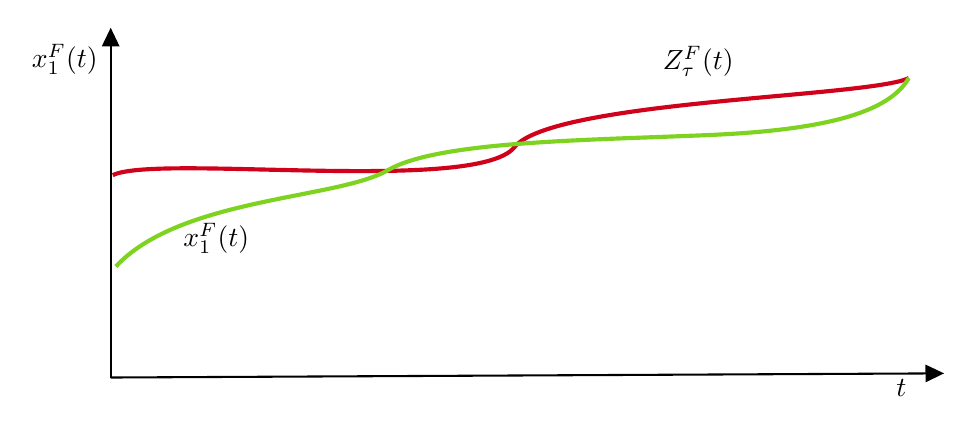
\begin{tikzpicture}[x=0.75pt,y=0.75pt,yscale=-1,xscale=1]
	%uncomment if require: \path (0,300); %set diagram left start at 0, and has height of 300
	
	%Curve Lines [id:da13273873192183094] 
	\draw [color={rgb, 255:red, 208; green, 2; blue, 27 }  ,draw opacity=1 ][line width=1.5]    (41.5,82.75) .. controls (62.66,72.39) and (217.06,91.85) .. (235,69.29) .. controls (252.94,46.73) and (406.16,45.22) .. (425,35.99) ;
	%Curve Lines [id:da36265400331191766] 
	\draw [color={rgb, 255:red, 126; green, 211; blue, 33 }  ,draw opacity=1 ][line width=1.5]    (43,126.75) .. controls (74,93.46) and (149.94,94.37) .. (174,80.38) .. controls (198.06,66.38) and (268,66.02) .. (329,63.41) .. controls (390,60.8) and (416.31,51.01) .. (425,35.99) ;
	%Straight Lines [id:da7392955293030656] 
	\draw [line width=0.75]    (40.5,180.25) -- (439,178.26) ;
	\draw [shift={(442,178.25)}, rotate = 179.71] [fill={rgb, 255:red, 0; green, 0; blue, 0 }  ][line width=0.08]  [draw opacity=0] (8.93,-4.29) -- (0,0) -- (8.93,4.29) -- cycle    ;
	%Straight Lines [id:da9916362390165014] 
	\draw [line width=0.75]    (40.5,180.25) -- (40.5,14.75) ;
	\draw [shift={(40.5,11.75)}, rotate = 90] [fill={rgb, 255:red, 0; green, 0; blue, 0 }  ][line width=0.08]  [draw opacity=0] (8.93,-4.29) -- (0,0) -- (8.93,4.29) -- cycle    ;
	
	% Text Node
	\draw (417.5,179.47) node [anchor=north west][inner sep=0.75pt]    {$t$};
	% Text Node
	\draw (1,18.4) node [anchor=north west][inner sep=0.75pt]    {$x_{1}^{F}( t)$};
	% Text Node
	\draw (74,104.3) node [anchor=north west][inner sep=0.75pt]    {$x_{1}^{F}( t)$};
	% Text Node
	\draw (305,19.34) node [anchor=north west][inner sep=0.75pt]    {$Z_{\tau }^{F}( t)$};
	
	
\end{tikzpicture}